%%%%%%%%%%%%%%%%%%%%%%%%%%%%%%%%%%%%%%%%%%%%%%%%%%%%%%%%%%%%%%%%%%%%%
%% This is a (brief) model paper using the achemso class
%% The document class accepts keyval options, which should include
%% the target journal and optionally the manuscript type. 
%%%%%%%%%%%%%%%%%%%%%%%%%%%%%%%%%%%%%%%%%%%%%%%%%%%%%%%%%%%%%%%%%%%%%
\documentclass[journal=jacsat,manuscript=article]{achemso}
\SectionNumbersOn

\usepackage{graphicx} % Allows png images
\usepackage[version=3]{mhchem} % Formula subscripts using \ce{}
\usepackage{xcolor,latexsym,epsfig,amssymb,amsmath,color,subcaption,pictex,amsfonts,multicol}
\usepackage{tocloft}
\usepackage{setspace}
\usepackage{siunitx}
\newcommand*\mycommand[1]{\texttt{\emph{#1}}}
\newcommand{\etal}{{\it et al.}\ }
\newcommand{\re}[1]{\textcolor{red}{#1}}


%%%%%%%%%%%%%%%%%%%%%%%%%%%%%%%%%%%%%%%%%%%%%%%%%%%%%%%%%%%%%%%%%%%%%
%% Meta-data block
%% ---------------
%% Each author should be given as a separate \author command.
%%%%%%%%%%%%%%%%%%%%%%%%%%%%%%%%%%%%%%%%%%%%%%%%%%%%%%%%%%%%%%%%%%%%%

\author{Mazharul M. Islam}
\affiliation{Department of Chemistry, University of Bath, Claverton Down, Bath BA2 7AY, UK}
\alsoaffiliation{The Faraday Institution, Quad One, Becquerel Avenue, Harwell Campus, Didcot, OX11 0RA, UK}

\author{Lucy M. Morgan}
\affiliation{Department of Chemistry, University of Bath, Claverton Down, Bath BA2 7AY, UK}
\alsoaffiliation{The Faraday Institution, Quad One, Becquerel Avenue, Harwell Campus, Didcot, OX11 0RA, UK}

\author{Hui Yang}
\affiliation{Department of Materials, Imperial College London, London SW7 2AZ, UK}
\alsoaffiliation{The Faraday Institution, Quad One, Becquerel Avenue, Harwell Campus, Didcot, OX11 0RA, UK}

\author{Kieran O'Regan}
\affiliation{School of Metallurgy and Materials, University of Birmingham, Edgbaston, Birmingham, BT15 2TT, UK}
\alsoaffiliation{The Faraday Institution, Quad One, Becquerel Avenue, Harwell Campus, Didcot, OX11 0RA, UK}

\author{Anisha N. Patel}
\affiliation{Department of Mechanical Engineering, Imperial College London, London, SW7 2AZ, UK}
\alsoaffiliation{The Faraday Institution, Quad One, Becquerel Avenue, Harwell Campus, Didcot, OX11 0RA, UK}

\author{Abir Ghosh}
\affiliation{Department of Mechanical Engineering, Imperial College London, London, SW7 2AZ, UK}
\alsoaffiliation{Department of Chemical Engineering \& Technology, Indian Institute of Technology (BHU), Varanasi, Uttar Pradesh 221005, India}
\alsoaffiliation{The Faraday Institution, Quad One, Becquerel Avenue, Harwell Campus, Didcot, OX11 0RA, UK}

\author{Emma Kendrick}
\affiliation{School of Metallurgy and Materials, University of Birmingham, Edgbaston, Birmingham, BT15 2TT, UK}
\alsoaffiliation{The Faraday Institution, Quad One, Becquerel Avenue, Harwell Campus, Didcot, OX11 0RA, UK}

\author{Monica Marinescu}
\affiliation{Department of Mechanical Engineering, Imperial College London, London, SW7 2AZ, UK}
\alsoaffiliation{The Faraday Institution, Quad One, Becquerel Avenue, Harwell Campus, Didcot, OX11 0RA, UK}

\author{Gregory Offer}
\affiliation{Department of Mechanical Engineering, Imperial College London, London, SW7 2AZ, UK}
\alsoaffiliation{The Faraday Institution, Quad One, Becquerel Avenue, Harwell Campus, Didcot, OX11 0RA, UK}

\author{Benjamin J. Morgan}
\affiliation{Department of Chemistry, University of Bath, Claverton Down, Bath BA2 7AY, UK}
\alsoaffiliation{The Faraday Institution, Quad One, Becquerel Avenue, Harwell Campus, Didcot, OX11 0RA, UK}

\author{M. Saiful Islam}
\affiliation{Department of Chemistry, University of Bath, Claverton Down, Bath BA2 7AY, UK}
\alsoaffiliation{The Faraday Institution, Quad One, Becquerel Avenue, Harwell Campus, Didcot, OX11 0RA, UK}

\author{Jacqueline Edge}
\affiliation{Department of Mechanical Engineering, Imperial College London, London, SW7 2AZ, UK}
\alsoaffiliation{The Faraday Institution, Quad One, Becquerel Avenue, Harwell Campus, Didcot, OX11 0RA, UK}

\author{Aron Walsh}
\affiliation{Department of Materials, Imperial College London, London SW7 2AZ, UK}
\affiliation{Department of Materials Science and Engineering, Yonsei University, Seoul 03722, Korea}
\alsoaffiliation{The Faraday Institution, Quad One, Becquerel Avenue, Harwell Campus, Didcot, OX11 0RA, UK}
\email{a.walsh@imperial.ac.uk}

%\title[NMC]{Developments in Modelling of LiNi\textsubscript{x}Mn\textsubscript{y}Co\textsubscript{z}O\textsubscript{2} (NMC) Cathode Materials: from Atomistic to Continuum}

\title[NMC]{Multi-scale Modelling of LiNi\textsubscript{x}Mn\textsubscript{y}Co\textsubscript{z}O\textsubscript{2} (NMC) Cathodes for Li-ion Batteries: from Atoms to Cells}

% Reviews (by invitation only) are similar to Perspectives but offer a more comprehensive look at an emerging topic (6-10 journal pages). Authors of Reviews are encouraged to also submit a video (3-5 min clip) highlighting the theme of their Review. 
% https://publish.acs.org/publish/author_guidelines?coden=aelccp

\begin{document}
\singlespacing

\newpage

\begin{abstract}
The first generation of cathodes in commercial lithium-ion batteries are based on layered transition metal oxides. Research on ternary compounds such as LiCoO$_2$ evolved into mixed-metal systems, notably Li(Ni,Mn,Co)O$_2$ (NMC), which allows significant tuning of the physical properties. Despite its widespread application in commercial devices, the fundamental understanding of NMC is limited. Here, we review the latest insights from multi-scale modelling, bridging between the redox phenomena that occur at an atomistic level to the transport of ions and electrons across an operating device. We discuss changes in the electronic and vibrational structure through the NMC compositional space and how these link to continuum models of electrochemical charge/discharge cycling. Finally, we outline the remaining challenges for predictive models of high-performance batteries including capturing the relevant device bottlenecks and chemical degradation processes such as oxygen evolution. 
\end{abstract}

\begin{center}
    \includegraphics[width=8.25cm]{Figures/TOC.jpg} 
\end{center}

\clearpage

%\section{Introduction (all)}
% Rechargeable batteries – Li batteries, current uses, need to improve.
Lithium-ion batteries (LIBs) were first developed by Whittingham in the 1970s \cite{whittingham1974hydrated,whittingham1976electrical} but did not become a promising material until 1979 when Goodenough and Mizushima successfully demonstrated \ce{LiCoO2} as a cathode.\cite{mizushima1980lixcoo2} 
These were successfully commercialized by Sony in 1991 and have since become instrumental in portable electronics, electric vehicles, and grid storage applications.\cite{armand2008building,scrosati2011lithium,goodenough2013li,etacheri2011challenges,he2012layered,rozier2015li,dunn2011electrical} 
However, to fully electrify the transport and energy sectors further advancements in LIBs are required to achieve higher energy densities, better longevity, and lower cost. 
The performance of a battery is highly dependant on the choice of cathode material and the transition metals they are composed of.\cite{Sari2019,Julien2014,whittingham2008materials,bruce2012li}

% Introduce Cathode – limiting factor, composite materials (NMC).
\ce{LiCoO2} offered a number of attractive features including ease of synthesis, reversible lithium insertion, high specific energy density, and high thermal stability.\cite{gibbard1989high,plichta1989improved,noh2013comparison} 
However, its application was limited due to capacity fade and the cost/geopolitical issues of cobalt mining, which made large scale energy storage solutions impractical. \cite{mo_impact_2018,Banza2009}. 
Other oxide materials such as \ce{LiNiO2} and Li$_x$Mn$_2$O$_4$ were considered, however, they have their own challenges, such as the longevity and safety of \ce{LiNiO2}, \cite{min_comparative_2016} and Li$_x$Mn$_2$O$_4$ showing irreversible structural changes due to Jahn-Teller effects and low capacity \cite{tian_performance_2018}. Partial replacement of Co in \ce{LiCoO2} with Ni and Mn was considered, resulting in the layered oxide Li[Ni$_x$Mn$_y$Co$_z$]O$_2$, where $x+y+z=1$, commonly termed NMC, with subsequent numbers relating to the ratio of the transition metals.\cite{paulsen2000o2,paulsen20002, lu2001layered,rozier2015li} 
These NMC materials were able to achieve a more balanced performance, preserving favourable voltage characteristics, reaching a higher capacity (\SI{200}{mA.h.g^{-1}}), and addressing cost and abundance issues. \cite{sun_electronic_2017,larcher2015towards,ohzuku2001layered} 
NMC also demonstrates improved electrochemical performance, enhanced rate capability \cite{noh2013comparison,dahn1991rechargeable}, and better cycle life/thermal stability \cite{kim2006synthesis,armstrong1996synthesis}.

%Going to Ni rich and NMC811
The tuning of the transition metal (TM) compositions of NMC has been a focus of research, in an effort to optimise desirable battery properties including capacity, cyclic rate, electrochemical stability, and lifetime, whilst also reducing cost. \cite{duan2019insights} Most NMC compositions are already in use, with commercial applications shifting from NMC111 to higher Ni compositions including NMC811 (Li[Ni$_{0.8}$Mn$_{0.1}$Co$_{0.1}$]O$_2$). \cite{zhang2018structural} 
Current investigations are now focused towards further reducing the Co content and optimising NMC811 to improve the performance of current and future-generation batteries for long-range electric vehicles \cite{azevedo2018mining} and for use in all-solid-state LIBs. \cite{myung2017nickel,ohzuku_layered_2001, lu2001layered,belharouak2003li,kim2014unexpected,sun_electronic_2017}

%Challenges for NMC811 
Despite the improved properties of NMC811, the material still exhibits fast voltage and capacity fading as well as poor structural and thermal stability\cite{noh2013comparison,Li-aenm-2019,Jerng-ACS-AMI-2020}, which lead to severe degradation. \cite{Zhang-acs.chemmater-2019,Feng-2019,Xia2018,De-AdMat-2019,Li_Nat-Comm-2017,Manthiram-NatComm-2020} Degradation can occur through a range of physical and chemical processes resulting in loss of lithium inventory (LLI), loss of active material (LAM), and/or impedance increase.\cite{vetter2005ageing} 
Attempts have been made to circumvent these degradation processes using approaches including surface coating, doping with ions, and electrolyte modification;\cite{maleki2019controllable,Liu-JSSE-2020} however, current experimental probes are limited in the detail they can provide. 
Additional challenges lie in improving safety and prolonging life of batteries, which requires optimal thermal and operational management. 
This is where computational modelling can provide greater insight.

%Modelling techniques
Atomistic techniques, including Density Functional Theory (DFT) and classical Molecular Dynamics (MD), and continuum techniques, including the Doyle-Fuller-Newman (DFN) model and its simplification the single-particle model (SPM) \cite{Newman1975porous, Doyle1993DFN} broadly describe battery modelling techniques from atom to cell level. \cite{Howey_2020} 
DFT is well suited for investigating electronic structure, whereas MD, either \textit{ab-initio} or classical, can be used to provide vital information on system dynamics. These atomistic models can provide insights into material properties, however, they are limited by scale. 
Continuum modelling, a larger scale computational technique, is better placed to provide cell level properties. 
The DFN model assumes the electrodes are comprised of a homogeneous matrix of spherical particles and is able to predict the dynamics and internal states (Li concentration within active materials) of a battery. The SPM is a further simplification that considers one representative particle.
%In battery research these are the most commonly used continuum models due to their parameter requirements. This class of model is afforded accuracy, however computational expense currently precludes use in commercial applications including battery management systems. 
Combining atomistic and continuum model predictions, within a multi-scale modelling framework, can provide a more detailed understanding of the charge and mass transport processes, resulting in more accurate predictions of battery behaviour.

% review outline -  Motivation and what our review is about.
In this Review, drawn from our experience as part of the multi-scale modelling fast-start project of the Faraday Institution, we highlight the importance of modelling NMC across length and time scales. We also provide an outlook to current and future challenges faced in the modelling of NMC and other multi-component cathode materials.

%Firstly, we start at the atomistic scale, discuss the importance of transition metal oxide states and the roles they play in degradation processes, presenting work which has recently furthered this understanding. We discuss modelling of ion diffusion in NMC, presenting insight into the challenges posed by the material and the considerations needed for classical modelling. Continuing with the dynamics properties, we discuss vibrational structure and thermal transport in NMC, using the lattice dynamics of the crystalline material, discussing phonon dispersion and density, and the Jahn-Teller effect. We then move to the continuum scale, discussing the parameterisation of DFN models, key NMC degradation mechanisms and experimental characterisation techniques, and the modelling of degradation mechanisms of NMC electrodes specifically the phase transitions of the NMC surfaces during charging at higher state of charges (SOCs). 

\section*{Electrons: Oxidation State Competition}
The practical use of Ni-rich NMC materials in LIBs faces various challenges including structural degradation and capacity fading.  
The redox reactions and consequent reversible capacity of NMC are primarily influenced by the cation ordering and spin interaction of active elements in the TM layers. \cite{Li-acsami-2020,Maleki-aenm.2019,Feng-2019, Xia2018, Xiao_NanoEner2018}. 
Different compositions and charge distributions result in the appearance of various valence states, e.g. Ni$^{2+}$, Ni$^{3+}$, Ni$^{4+}$, Co$^{3+}$, Co$^{4+}$, Mn$^{4+}$. \cite{Xiao_NanoEner2018} 
The coexistence and interactions of these multivalent TM chargess and spins make it difficult to determine a unique ground state for NMCs. \cite{Xiao_NanoEner2018}
Understanding the range of transition metal oxidation states, and the roles they play in degradation processes, is therefore crucial for the improvement of these promising cathode materials.

Ni is a key redox active element in NMC. Experimentally, Ni in NMC811 is present as a mixture of Ni$^{2+}$ (with electronic configuration of ${t_{2g}}^{6}{e_{g}}^{2}$) and Ni$^{3+}$ (${t_{2g}}^{6}{e_{g}}^{1}$) oxidation states, with an average value close to 3+. \cite{Zhu_JMatChemA2019,Katharina-chemmater,Kondrakov_JPhysChemC2017} 
During charging-discharging cycling, the Ni$^{2+}$  can migrate from the Ni plane (3a) to the Li plane (3b), creating a Li/Ni disorder. \cite{Zhang-acs.chemmater-2019, Feng-2019, Xia2018} This leads to a structural transformation (layered to defect spinel/disordered rock-salt transition) and blocks the Li$^{+}$  migration channels.\cite{Xia2018} Ni$^{4+}$ (${t_{2g}}^{6}{e_{g}}^{0}$) 
This is thought to be the origin of cracking and subsequent performance degradation upon lithium extraction.\cite{Katharina-chemmater,Li-aenm-2019,Li-EER-2020}   
The dissolution of NMC, resulting in capacity attenuation, can occur due to the TM disproportionation.\cite{buchberger2015} 
Ni disproportionation in pristine NMC811 has not been reported experimentally. 
In a previous computational study \cite{HChen_PhysRevB2011}, $2$Ni$^{3+}\rightarrow$Ni$^{2+} + $Ni$^{4+}$, has been discussed for LiNiO$_2$. 
Charge disproportionation is observed in other cathode materials such as in pristine LiMn$_2$O$_4$ where  $2$Mn$^{3+}\rightarrow$Mn$^{2+} + $Mn$^{4+}$ disproportionation is considered to be the main responsible for Mn dissolution. Elucidation of active metal disproportionation in NMCs is important as it poses a threat of poisoning the anode \cite{Parmar-LMO-2020,PASQUALINI2017} and forming inorganic layers in SEIs \cite{joshi2014}, which in turn lead to the capacity fading. 

The complex ordering and multivalent nature of transition metals poses significant challenges for modelling.
Previous theoretical investigations have studied the influence of oxidation states on various properties of NMC materials. \cite{Dan-Thomas-chemmater,Sun_JPhysChemC2017,Dixit_JPhysChemC2017,Hoang_ACSChemMater2016,Dixit_JElecSoc2017}  These studies, employing the DFT+\textit{U} approach to treat the high correlation of the TM 3d orbitals, have calculated Jahn-Teller distortion effects, atomic magnetic moments and density of states for the elucidation of TMs oxidation states. 
Ni$^{2+}$ is predominant over Ni$^{3+}$ in NMC333, NMC442, and NMC532, whereas with the increase of Ni content, the occupation of Ni$^{3+}$ steadily increases at the cost of Ni$^{2+}$. 
In NMC811, the Ni$^{3+}$  fraction is up to 58 \%. \cite{ Sun_JPhysChemC2017} 
The presence of Ni$^{4+}$ is observed at delithiation conditions and the concentration increases rapidly in Ni-rich NMC materials as a function of Li content. \cite{Dixit_JPhysChemC2017} 
Sun and Zhao \cite{ Sun_JPhysChemC2017} have reported the existence of Co$^{2+}$ ions along with Co$^{3+}$  ions in pristine NMCs, which was opposed by \citeauthor{Dixit_JPhysChemC2017}\cite{ Dixit_JPhysChemC2017}. 
Based on magnetic moments and PDOS calculations it was concluded that Co remains as Co$^{3+}$ in different pristine NMCs. Mn$^{4+}$ remains in close proximity to Ni$^{2+}$ which influences the super-exchange interactions among transition metals. \cite{zheng2019} In NMC materials with mixed valence states of Ni$^{2+}$/ Ni$^{3+}$, Ni$^{3+}$  has the priority to exchange with Li and changes to a Ni$^{2+}$ state with a spin-flip, to form strong linear Ni$^{2+}$–O2–– Ni$^{2+}$ /Mn$^{4+}$ super-exchange networks. 
This acts as the driving force in tuning the Ni/Li disordering. \cite{zheng2019,Zheng-acs.jpclett-2017} 

%
% AW - IS THIS A REVIEW OR NEW RESULTS? - LM this is a review of work currently in progress to be submitted "soon".
% I DIDNT EDIT THIS SECTION YET
%
Recently, \re{\citeauthor{rana}} have employed HF-DFT hybrid HSE06 functional coupled with Wannier function analysis to assign oxidation states in Ni rich NMC811 (LiNi$_{0.8}$Mn$_{0.1}$Co$_{0.1}$O$_{2}$). \cite{rana} The effect of transition metal ordering and oxidation state configuration on the relative stability of different NMC811 models was studied. The limitations of other approaches to assign oxidation states, such as analysis of magnetic moments and Jahn-Teller distortions, were also illustrated.

%\subsection{Stability and Oxidation State Distribution in NMC-811}
By randomly varying the atomic positions of Ni, Mn and Co in the lattice, \re{\citeauthor{rana}} created 50 structural models of NMC811. The total energy values of these structures were calculated by full optimization of the fractional coordinates and the lattice parameters. The calculated energies depend on the transition metal arrangement, resulting in preferred TM configurations. This finding is in contrast to recent suggestions that the transition metal cations in NMC811 are randomly distributed. \cite{Sun_JPhysChemC2017} The stability of the NMC811 varies due to the distribution and interaction of mixed oxidation states of the TM ions (Ni$^{2+}$/Ni$^{3+}$/Ni$^{4+}$, Co$^{3+}$, and Mn$^{4+}$). This is in line with the experimental observations that the spin interactions of TM ions influence the ground state stability of NMC. \cite{Xiao_NanoEner2018}  Figure \ref{fig:stability}(a) presents the proportion of Ni ions in a given oxidation state for all considered models obtained with the HSE06 functional, ordered by relative energies per formula unit. \cite{rana} 

The distribution of transition metals is the only difference between these 50 NMC811 models. Therefore, it is clear that the relative energies of NMC811 structures depends strongly on how the mixed oxidation state transition metals are ordered and the interactions between them.

\begin{figure}[tb]
  \begin{center}
  \begin{tabular}{c c}
  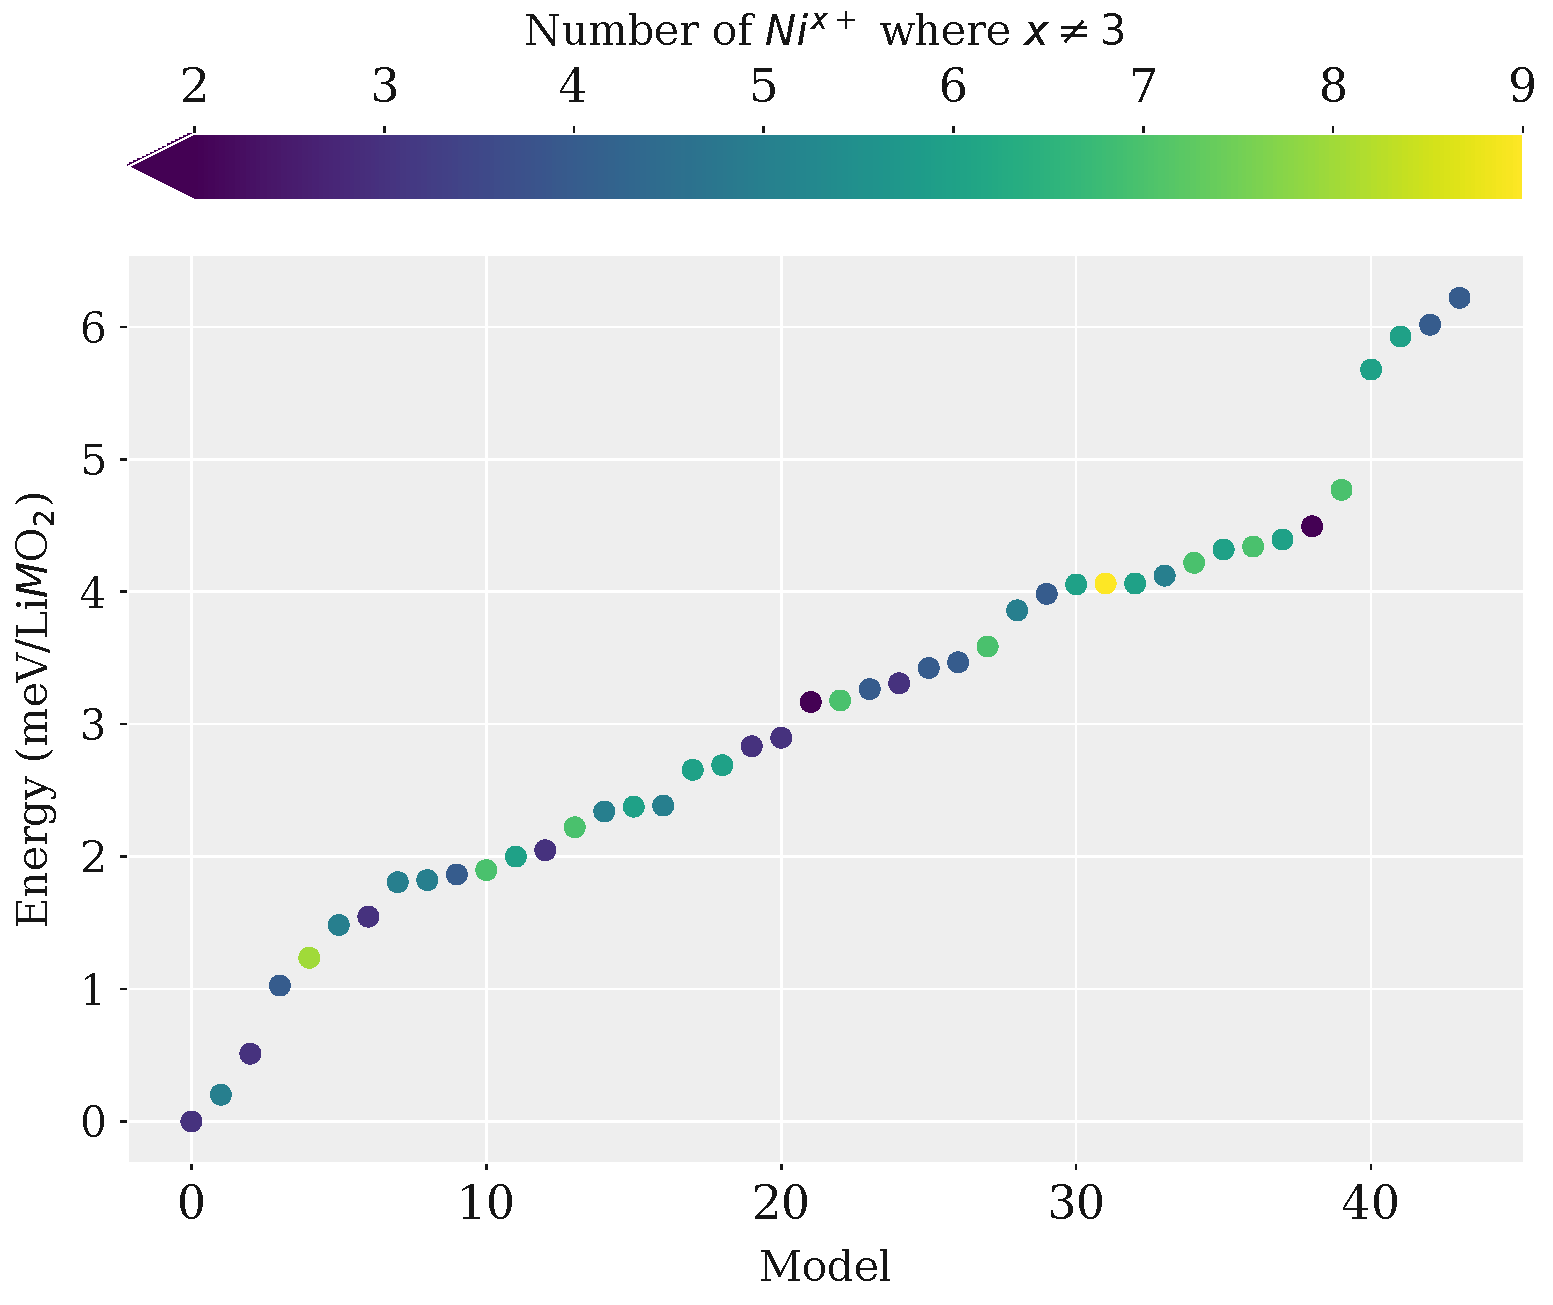
\includegraphics[width=0.46\columnwidth]{Figures/HSE_energy_cmap.pdf}&\includegraphics[width=0.46\columnwidth]{Figures/Ni_ox_vs_E.pdf}\\
  \textbf{(a)}&\textbf{(b)}\\
%    \includegraphics[width=0.75\columnwidth]{Ni_ox_vs_E.pdf}
   \end{tabular}
    \caption{\label{fig:stability} \textbf{(a)} Relative stabilities of different NMC-811 structural models obtained with the HSE06 functional, and the deviation in number of Ni$^{3+}$ in the material from the ``simple'' oxidation state model of \{1 Ni$^{2+}$;7 Ni$^{3+}$; 1 Mn$^{4+}$; 1 Co$^{3+}$\}, which would have 21 Ni$^{3+}$ for the supercell. \textbf{(b)} \% of Ni ion by oxidation state for each model, versus the relative energy per atom of the NMC model calculated with the HSE06 functional. Reproduced with permissions from \citenum{rana}. }
    \end{center}
\end{figure}

The analysis of the \% of Ni shows a mixture of Ni states, Figure \ref{fig:stability}(b). Nickel in NMC811 has been reported as having a mix of Ni(II/III) oxidation states, with the average value close to 3+, \cite{Zhu_JMatChemA2019,Kondrakov_JPhysChemC2017} which could potentially be rationalised by a simple distribution \{1 Ni$^{2+}$;7 Ni$^{3+}$;1 Mn$^{4+}$; 1 Co$^{3+}$\} oxidation state model. Several instances of this simple oxidation state distribution was found within \citeauthor{rana}'s data set. The two lowest energy structures here account for this oxidation state distribution. On examining the transition metal ordering in these lowest energy structures it can be seen that Mn$^{4+}$ and Ni$^{2+}$ lie in adjacent 3b sites along the shortest crystal axis. It forms continuous linear chains of alternating Mn$^{4+}$-Ni$^{2+}$ throughout all transition metal layers. This long range linear chain ordering is consistent with local charge balance, as discussed by \citeauthor{Zeng_ChemMater2007} \cite{Zeng_ChemMater2007}. As the two lowest energy structures contain this transition metal ordering, it suggests that the main stabilising effect of these models are the result of extended Mn$^{4+}$-Ni$^{2+}$ coordination. However, it should be noted that with the increase of supercell size, the probability of Mn$^{4+}$-Ni$^{2+}$ residing next to each other might reduce.

In a large proportion of NMC811 configurations \citeauthor{rana} investigated, $2$Ni$^{3+}\rightarrow$Ni$^{2+} + $Ni$^{4+}$ disproportionation is also observed. This occurs in some of the most stable structures in the data set, for example see the third most stable model in Figure \ref{fig:stability}(b). It can therefore be concluded that $2$Ni$^{3+}\rightarrow$Ni$^{2+} + $Ni$^{4+}$ disproportionation occurs in the pristine NMC811 structure before charging, illustrating that Ni$^{4+}$ is present in the fully lithiated material rather than only appearing on lithium deintercalation.

%Analysis of the Jahn-Teller (JT) distortion effects is a popular approach for the identification of the oxidation states. Recently, Sun and Zhao have determined the oxidation states of TMs in NMC by analysing the JT effect and TM–O bond length. \cite{Sun_JPhysChemC2017} In \citeauthor{rana}, it was clearly demonstrated that JT distortion is not adequate to unambiguously assign the TMs oxidation states. The low-spin Ni$^{3+}$ state with a singly occupied orbital at the $e_{g}$ level is a JT active species. In Figure \ref{fig:JT}, the calculated Ni--O octahedral bond lengths found within \citeauthor{rana}'s data set are presented. It is observed that while it is possible to identify Ni$^{3+}$-O Jahn-Teller distorted complexes within the entire data set, the transition metal ordering leads to competition between local strain effects and Jahn-Teller distortion. The amount of distortion varies significantly. Therefore it is difficult to assign the oxidation states by distortion alone.  

%\begin{figure}[tb]
%  \centering
%  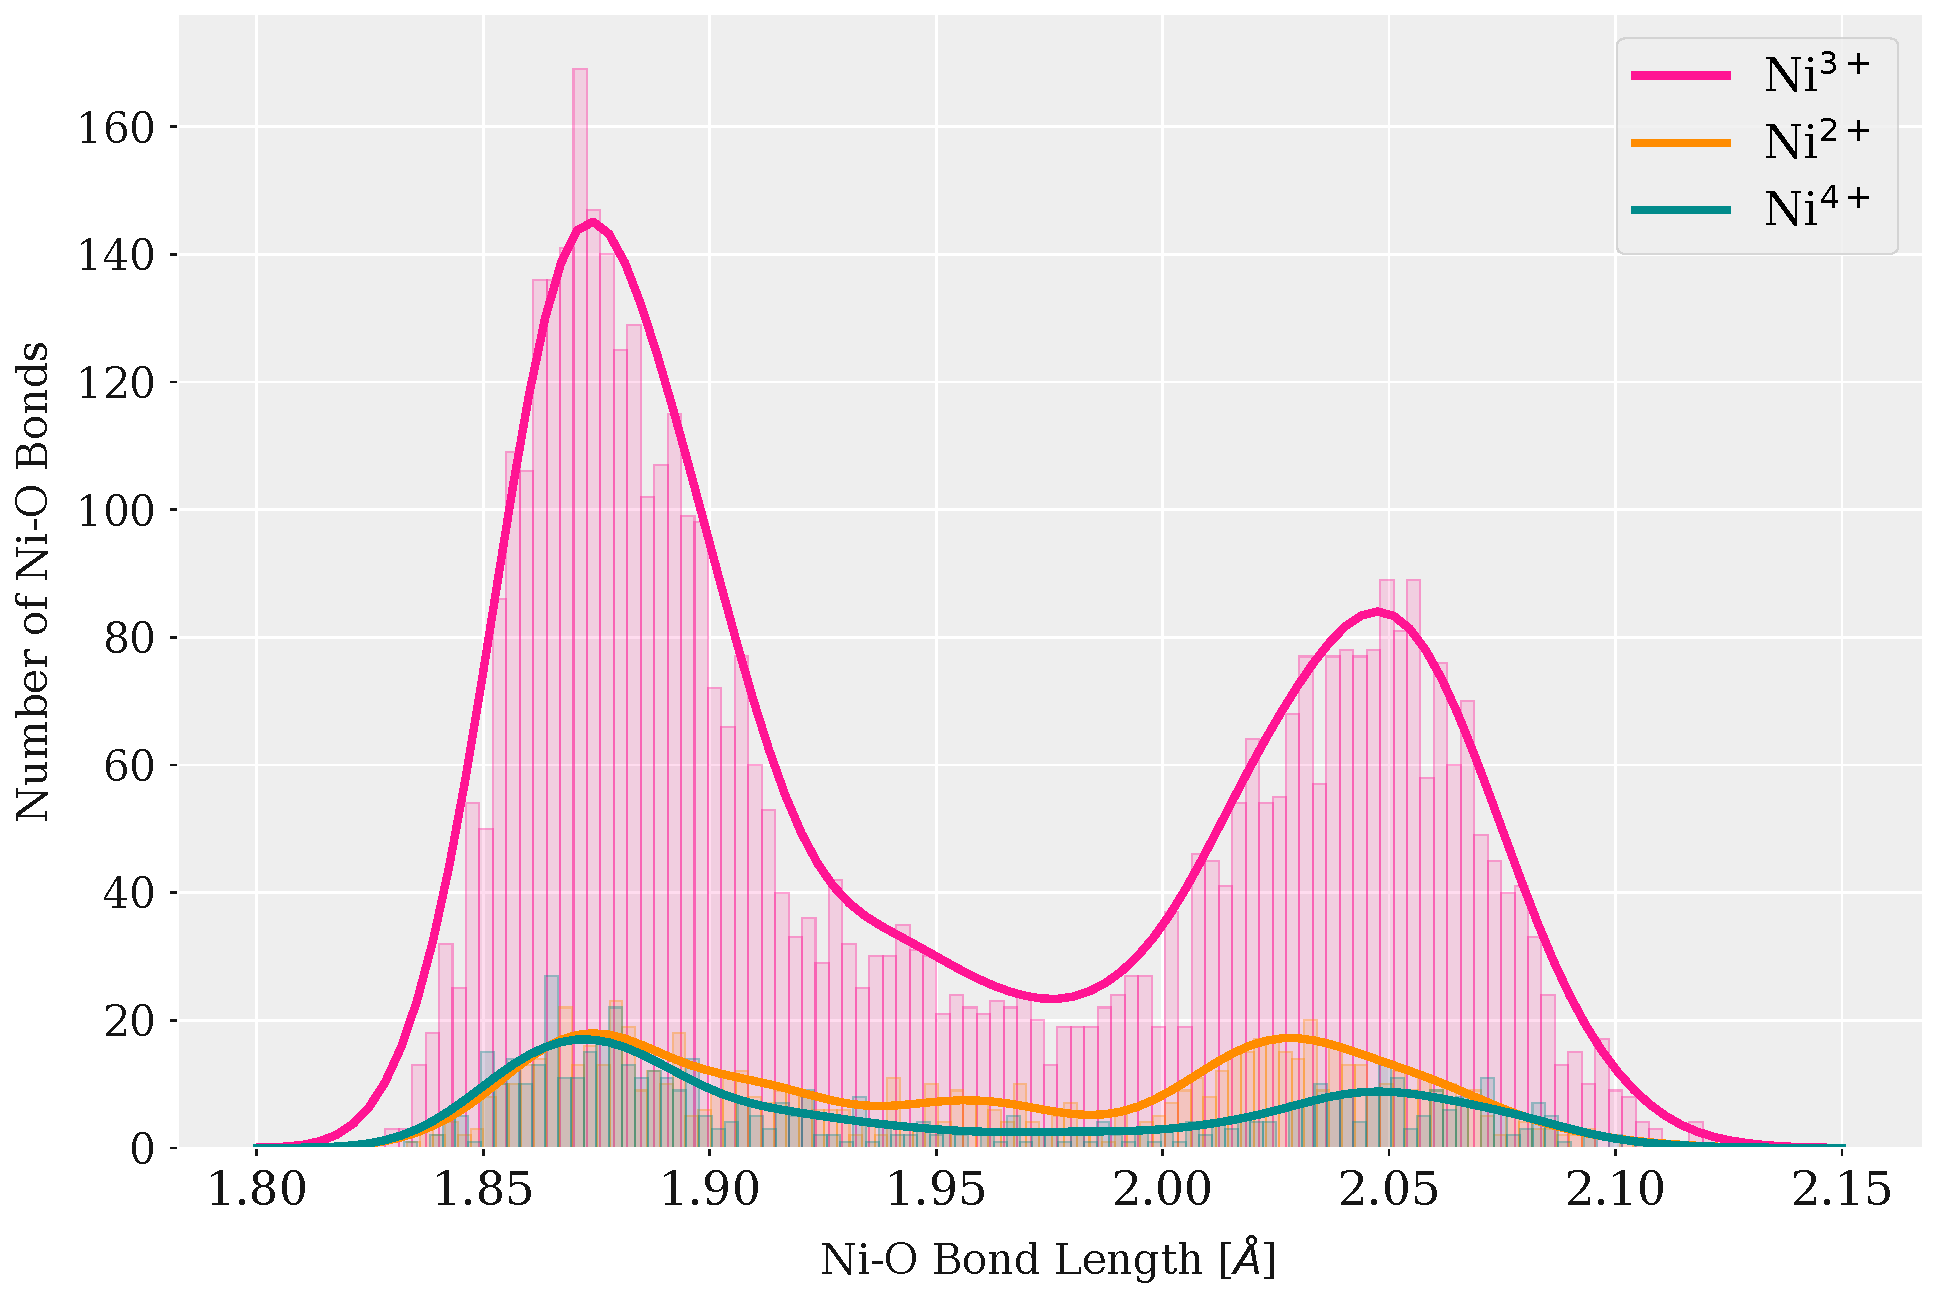
\includegraphics[width=0.75\columnwidth]{Figures/JT_all.pdf}
%    \caption{\label{fig:JT} Histogram showing Ni-O octahedral bond lengths separated by Wannier function assigned oxidation state, along with a Gaussian kernel density estimation. Reproduced with permissions from \citenum{rana}.}
%\end{figure}

%Calculation of atomic magnetic moment is another approach to assign oxidation states which was employed in previous computational studies. \cite{Dixit_JPhysChemC2017, Zheng-acs.jpclett-2017}. 
%In fig.\ \ref{fig:Mag}, the calculated atomic magnetic moments for all Ni ions in \citeauthor{rana}'s data set are presented. It is observed that there is a 
%continuous range of magnetic moments which highlights the ambiguity inherent in this approach.
%This may lead to incorrect assignment of oxidation states in some cases.
%For example, as shown in fig.\ \ref{fig:Mag} (b), the Wannier functions assigned to a Ni ion in one of the structures has a clear ${t_{2g}}^{6}{e_{g}}^{2}$ electronic configuration corresponding to Ni$^{2+}$. \citeauthor{rana} But DFT calculated magnetic moment was found in the range of low spin Ni$^{3+}$ as shown in the central region of fig.\ \ref{fig:Mag}(a).\citeauthor{rana} This demonstrates that magnetic moment can not always assign oxidation state correctly.

%\begin{figure}[tb]
%  \begin{center}
%  \centering
%  \begin{tabular}{c c}
%   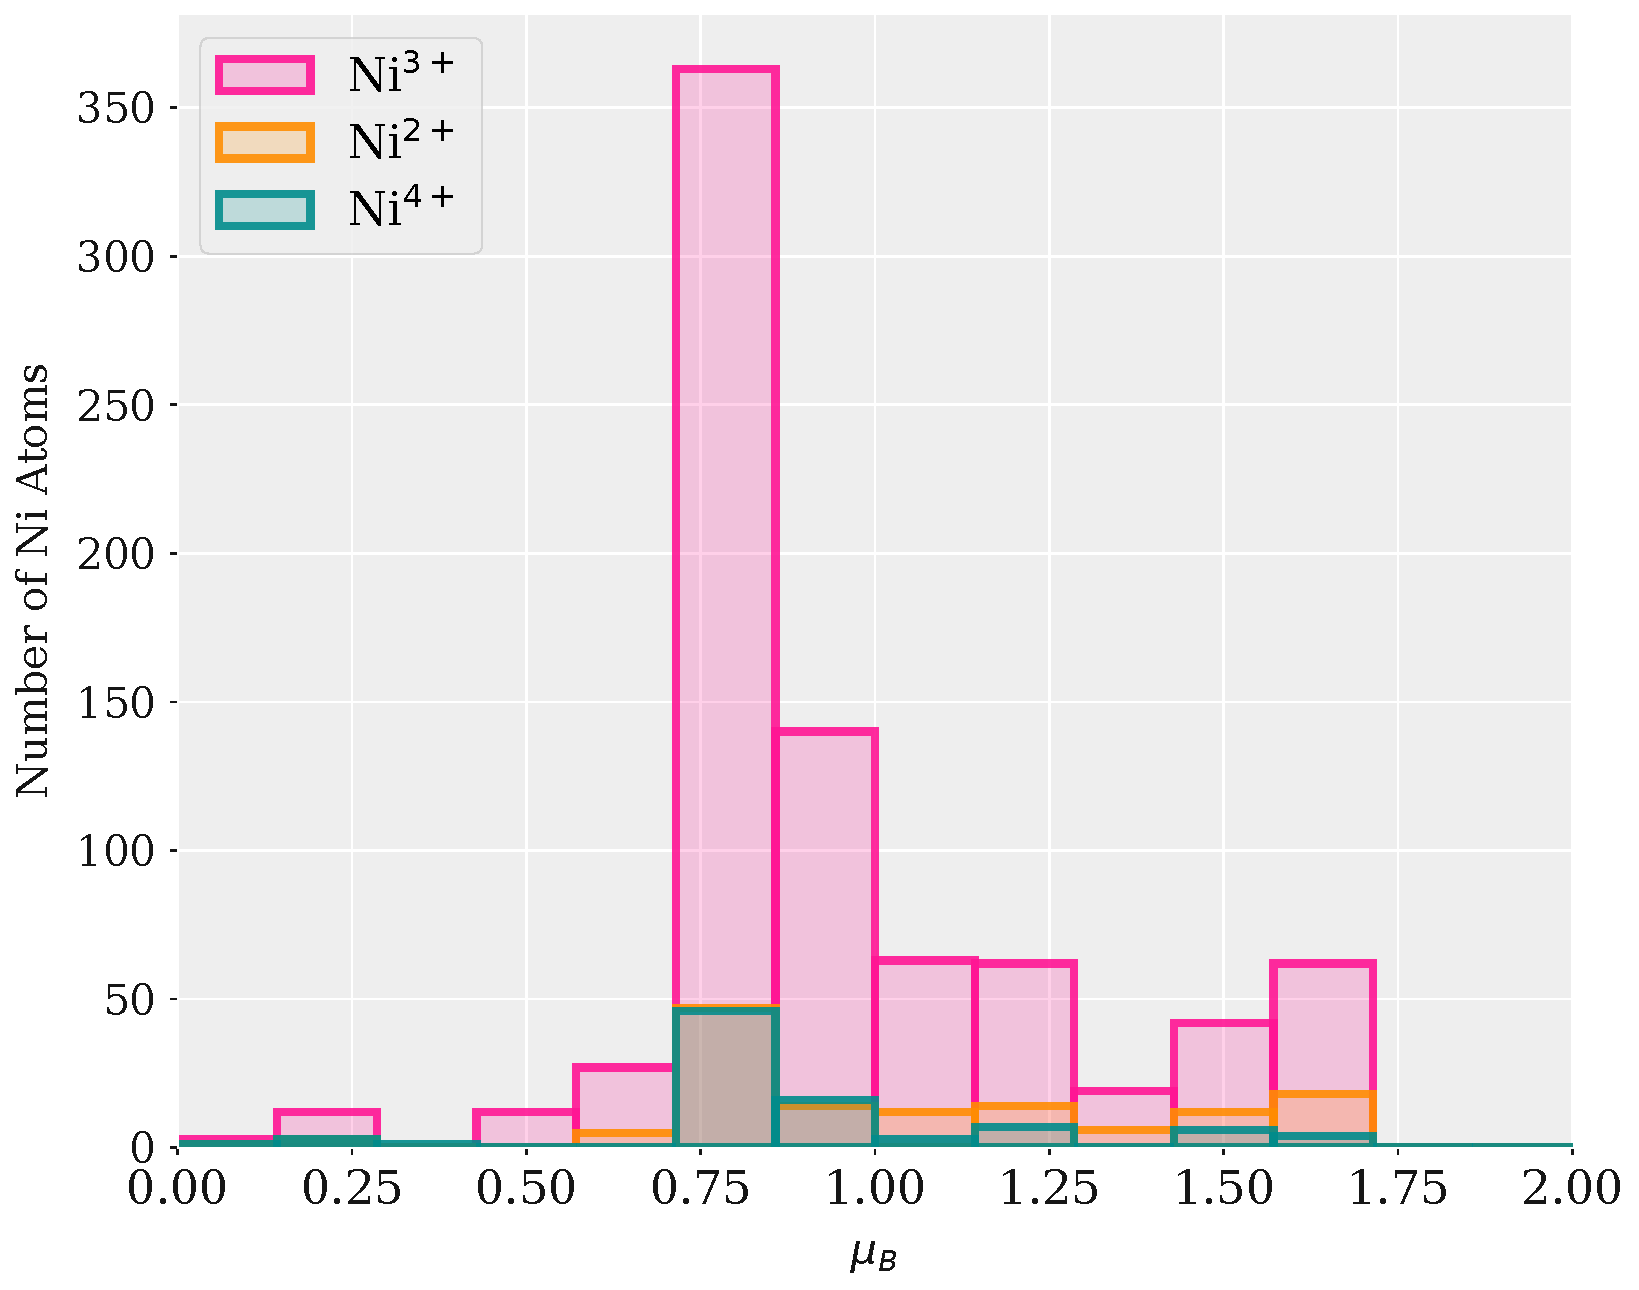
\includegraphics[width=0.5\columnwidth]{Figures/mag_mom_hist.pdf}&\includegraphics[width=0.4\columnwidth]{Figures/wannier_centres_assigned.pdf}\\
%  \textbf{(a)}&\textbf{(b)}\\
%   \end{tabular}
%    \caption{\label{fig:Mag} \textbf{(a)} Distribution of calculated magnetic moments, separated by Wannier assigned oxidation state \textbf{(b)} Ni$^{2+}$-O octahedra along with calculated Wannier functions, and occupations, for a selected Ni ion in a ${t_{2g}}^{6}{e_{g}}^{2}$ electronic configuration. Cyan and orange iso-surfaces illustrate positive and negative Wannier function components respectively. Reproduced with permissions from \citenum{rana}.}
%    \end{center}
%\end{figure}

This study \citenum{rana} showed that the transformation of Kohn-Sham electronic states to Wannier functions and then using the centre of gravity to associate each with an ion gives the most unambiguous description of oxidation states in NMC811. The findings from this study are important for the improvement of electrochemical behaviour of cathodes as well as for the understanding of structural degradation of LIBs during cycling. Further studies on the effects of delithiation and doping on transition metal oxidation states are currently underway to extend the understanding of NMC materials.

%\clearpage
\section*{Ions: Models of Diffusion}
%\subsection*{Interatomic Potentials}
Understanding ion diffusion is crucial for the development of batteries with high‐power density, especially in solid electrodes which present slow ion diffusion compared to electrolytes. 
The rate of diffusion can be understood through the diffusion coefficient, $D$. 
DFT is well suited to investigate local hopping mechanisms;\cite{van_der_ven_layered_2001, van_der_ven_LiTiS2_2008} however, when it comes to long range diffusion classical MD is better suited in terms of longer time- and length-scales. 
Here, the chemical bonding is described using interatomic potentials. 
There are many forms of interatomic potentials, with the ability to describe heteropolar solids such as NMC. 
The most widely used form for investigating diffusion properties is the Coulomb-Buckingham potential. \cite{buckingham_classical_1938} 
This is derived from the Born model\cite{born_1932, mayer_1932}, where the potential energy of the system is expressed as:
%
\begin{equation}
    E(r_{ij}) =  \sum_{ij} \frac{Q_i Q_j}{4\pi \varepsilon_0 r_{ij}} + \sum_{ij} A \ exp(\frac{-r_{ij}}{\rho}) - Cr_{ij}^{-6}
\end{equation}
%
Here, $i$ and $j$ are ions of charge $Q_i$ and $Q_j$ at a distance of $r_{ij}$ and $\varepsilon_0$ is the permittivity of free space. In the second term $A$, $\rho$, and $C$ are the parameters associated with the Buckingham potential.

The sole classical MD study reported for NMC111 employed core-shell Buckingham potentials. \cite{Lee_and_Park_2012}
Using these potentials for a range of NMC compositions, however, presented  catastrophic structural collapse upon removing Li (Figure \ref{fig:structure_collapse}). Ni in NMC111 is Ni$^{2+}$, whereas in delithiated structures and other compositions, other oxidation states, such as Ni$^{3+}$ arise. Similarly, delithiation results in the formation of mixed Ni oxidation states and charge disproportion, which is challenging to represent in a classical model. \cite{Nakamura_2019,Kim_2002,Alonso_1999} 
The complex nature of Ni chemistry extends to the LiNiO$_2$ ternary system. To the best of our knowledge, no interatomic potentials exist for Ni$^{3+}$, evidenced by a lack of classical MD publications for LiNiO$_2$ and NMC systems.

\begin{figure}[h]
  \centering
  \resizebox{16cm}{!}{\includegraphics*{Figures/structure_collapse.pdf}} %
    \caption{\label{fig:structure_collapse} Structure images for fully lithiated (centre) and 20 \% delithiated (right) NMC811 after an initial equilibration MD simulation using potentials from \citeauthor{Lee_and_Park_2012} (left). \cite{Lee_and_Park_2012} }
\end{figure}

%\subsection*{Developing Interatomic Potentials}
The development of interatomic potentials, which requires model paramaterization with respect to a set of target observables is a difficult task for systems of such complexity.  
For layered structures, variations of the Buckingham potentials have been developed, some using rigid ion models,\cite{Lewis_1985, Ledwaba2020, Sayle2005, Dawson2014} and others using core-shell models, \cite{Hart1998, Fisher2010, Lewis_1985,Ammundsen1999, Kerisit2014, He2019,lee2012atomistic} with a mixture of formal and partial charges.
Attempts were made to apply the fitting routines from established codes including the General Utility Lattice Program (GULP), \cite{gale_gulp_1997} Atomicrex, \cite{Stukowski_2017} dftfit, \cite{dftfit} and potfit. \cite{wen_kim-compliant_2017} 
Each codes poses unique functionality, however, none were able to produce robust potentials for NMC or LiNiO$_2$.
POtential Parameter Optimisation for Force-Fields (PopOff),\cite{Morgan2020PopOff} has been specifically developed within the Faraday Institution for fitting different permutations of the Buckingham potential. Its modular design allows flexible fitting of both rigid ion and core-shell models, and formal and partial charges. Here, we review important aspects determined to be vital when fitting cathode potentials using this code.

In systems such as NMC and LiNiO$_2$ the short-range interactions are overwhelmed by the longer-range Coulombic term. 
In these cases, the system charges need to be scaled down to increase the influence of the short-range interactions, termed as partial charges. 
A scaling factor of 60 \% formal charge is commonly used, \cite{pedone2006potentials} however, partial charges are system dependant. 
Figure \ref{fig:LiNiO2_fitting} (a) shows $\chi^2$ (fit error) for a fitted Buckingham potential for LiNiO$_2$ reducing with the charge scaling factor until approximately 60 \% of the formal charge, where it starts to plateau.
This is in broad agreement with literature, with a slightly improved fit at $\sim$50 \% formal charge.

\begin{figure}[h]
    \centering
    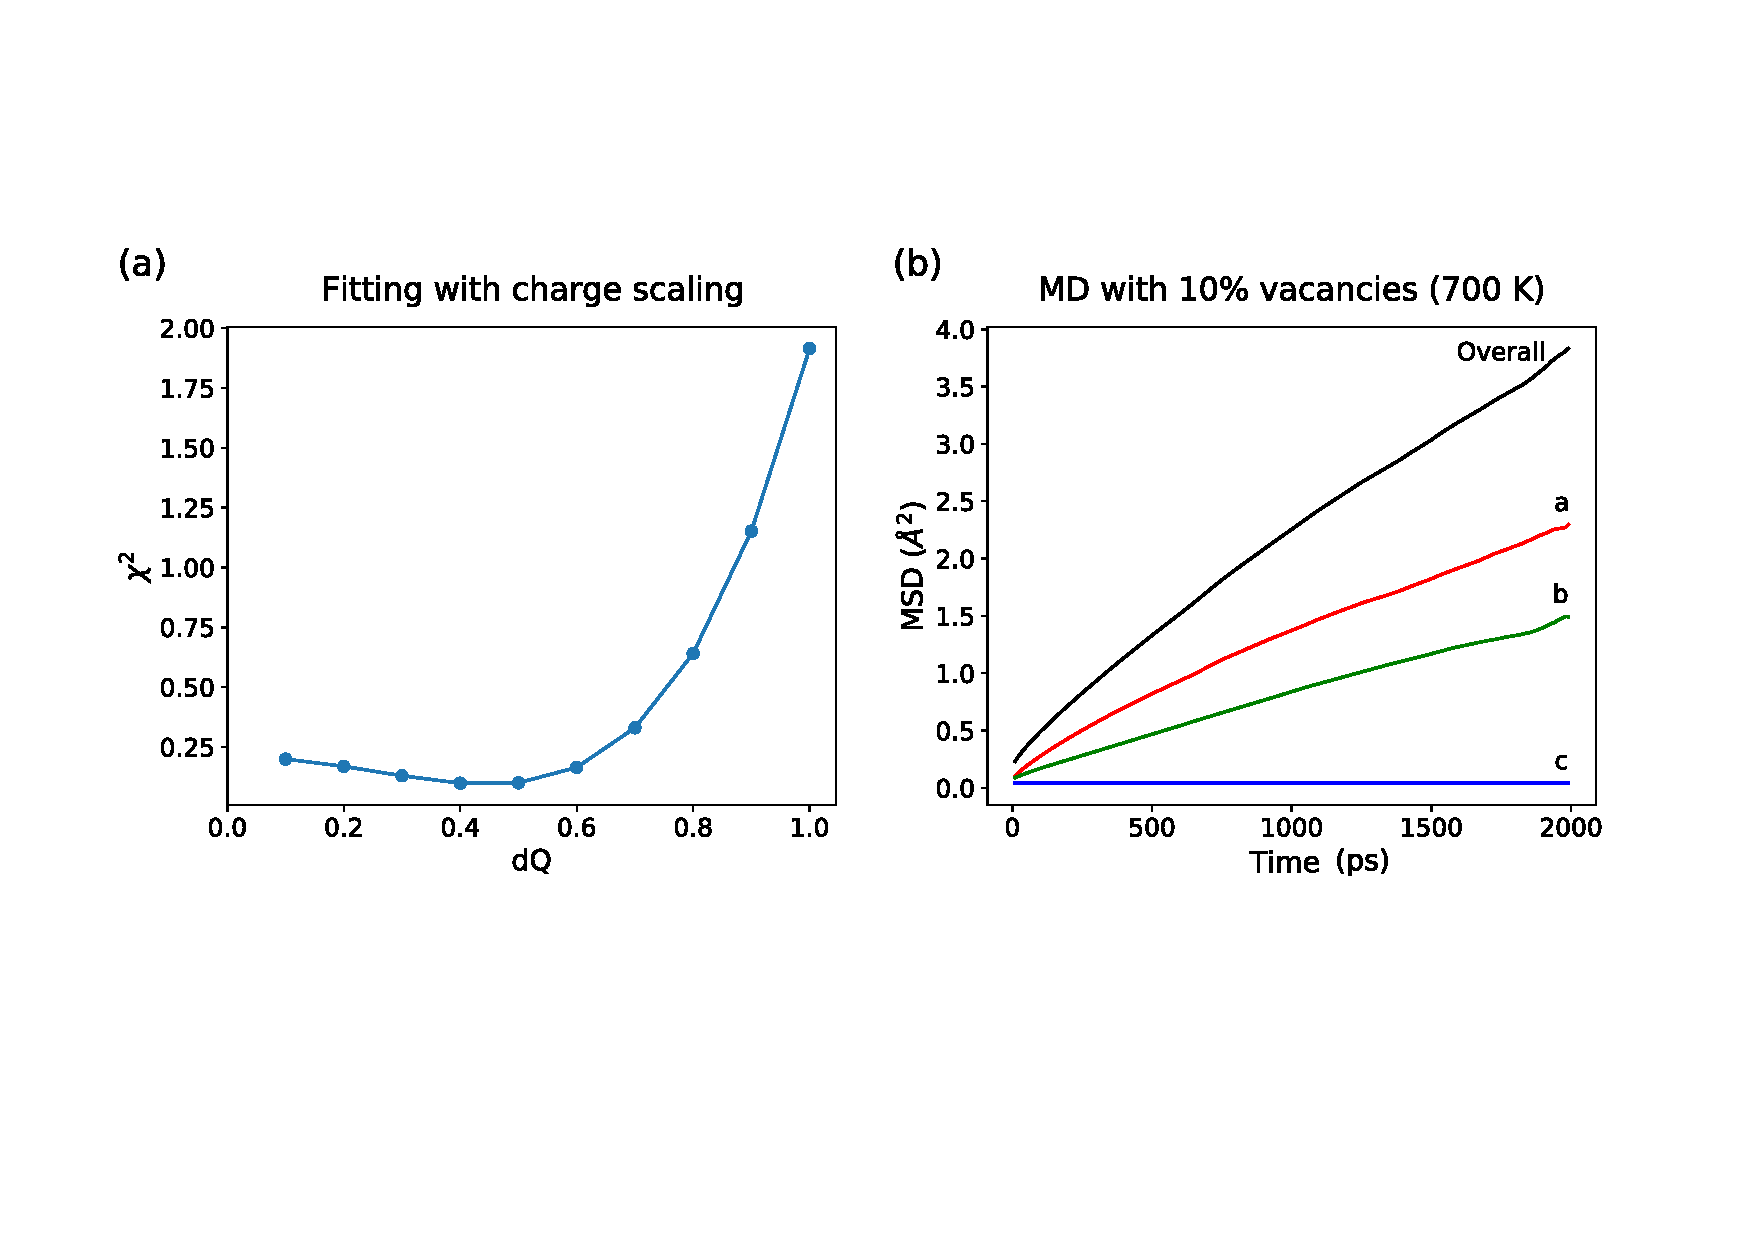
\includegraphics[scale=0.5]{Figures/LiNiO2_plots.pdf}
    \caption{\label{fig:LiNiO2_fitting} (a) Plot of the fit error, $\chi^2$, of LiNiO$_2$ as a function of the charge scaling factor, dQ, and (b) Plot of the mean squared displacement (MSD) of Li in LiNiO$_2$ with 10 \% Li vacancies at 700 K. As this is a layered material, it is expected that no movement will occur in the c direction, only in a and b.}
\end{figure}

Core-shell models introduce polarizability into classical MD simulations. The adiabatic shell model \cite{Mitchell_1993} has been widely used for calculating long trajectories. 
A fraction of the atomic mass is assigned to the shell and there is no explicitly defined fraction size; however, placing 10 \% of the atomic mass on the shell is commonly adopted. \cite{PLIMPTON19951,todorov2006dl_poly_3}

Fitting rigid ion potentials for LiNiO$_2$ (with partial charges) resulted in a fit error of $\chi^2$ = 1.665.
By introducing a core-shell potential on the oxygen, with Li and Ni remaining rigid ion, $\chi^2$ was reduced to 0.372. 
Presenting evidence that a core-shell potential is required to more accurately reproduce the forces and physics of the system.
In the case of the oxygen core-shell the spring constant was determined to be 15.443 eV $\cdot$\AA$^{-2}$, with a charge of -1.48 e on the shell and 0.520 e on the core.
Here, the best fit (lowest $\chi^2$) was a core-shell model on the oxygen in a partial charged system. The resulting potential was used with a 10 \% delithiated LiNiO$_2$ supercell to conduct MD studies at 700 K on the diffusion within the material.
The MSD, Figure \ref{fig:LiNiO2_fitting} (b), presents small movement of Li, however, the resulting self-diffusion coefficient, 6.664$\times 10^{-8}$  cm$^{2}$ s$^{-1}$, is within the measured range. \cite{Nakamura2000,bruce1992vacancy}
These results indicate that core-shell and partial charges are necessary to include in interatomic potential models for these systems. 

This highlights the careful consideration needed when fitting interatomic potentials for heteropolar solids such as NMC.
Fitting parameters also need to be tailored to the type of study being conducted.
For example, if the potentials for a cathode material were fitted only to lattice parameters, elastic constants, and the bulk modulus, then the potential would not be accurately representative of the cathode redox properties. 
If properties such as the dielectric constant were included, then redox chemistry would be better represented. 
Other features such as charge equilibrium and ligand field effects should also be considered. 
Fitting to every material property is not feasible, however, fitting to a broad range of the most relevant properties to the study is needed. 
Tools are currently in development to make fitting interatomic potentials more accessible to atomistic modellers. \cite{gale_empirical_1996, Stukowski_2017, wen_kim-compliant_2017, Morgan2020PopOff}

\section*{Phonons: Thermal Transport}
A traditional image of crystals is that of atoms being held in static positions through stiff chemical bonds. 
In reality, atoms are constantly vibrating around their average crystallographic positions in even the hardest of crystals. 
Lattice dynamics, based on calculation of the interatomic force constants in a crystal, is a powerful tool to model thermal effects from heat capacity to thermal expansion.
Recently, the description of anharmonic effects including vibrational lifetimes and thermal conductivity has become possible.

There have been a number of studies on the thermal properties of NMC. 
Recently, \citeauthor{yang2020chemical} reported the harmonic phonon dispersion for the \ce{LiMO2} (M = Ni, Co, Mn) endpoints in the NMC oxide system. \cite{yang2020chemical}
Their results revel that the Jahn-Teller (JT) effect is more pronounced in the crystalline \ce{LiMnO2} with three distinct bond lengths for the TM-O bonds. They found that the medium and low frequency modes are mainly due to motion of Li and TMs, while the high frequency modes ($>$ 14 THz) are vibrations involving the TM and O atoms.
The phonons also provide information of a group, theoretic analysis within the group assigns the irreducible representations of the acoustic and optic branches. Of these, some modes are infra-red (IR) active or Raman active, which is comparable with experimental IR/Raman spectra, with differences likely due to the volume expansion at finite temperature. \cite{yang2019highly} 
For NMC alloy systems, \citeauthor{sun_electronic_2017} showed that longitudional acoustic mode frequency increases from NMC333 to NMC811 (Figure \ref{figure_phonon}) due to the weaker electron screening.\cite{sun_electronic_2017}

\begin{figure}[]
  \centering
    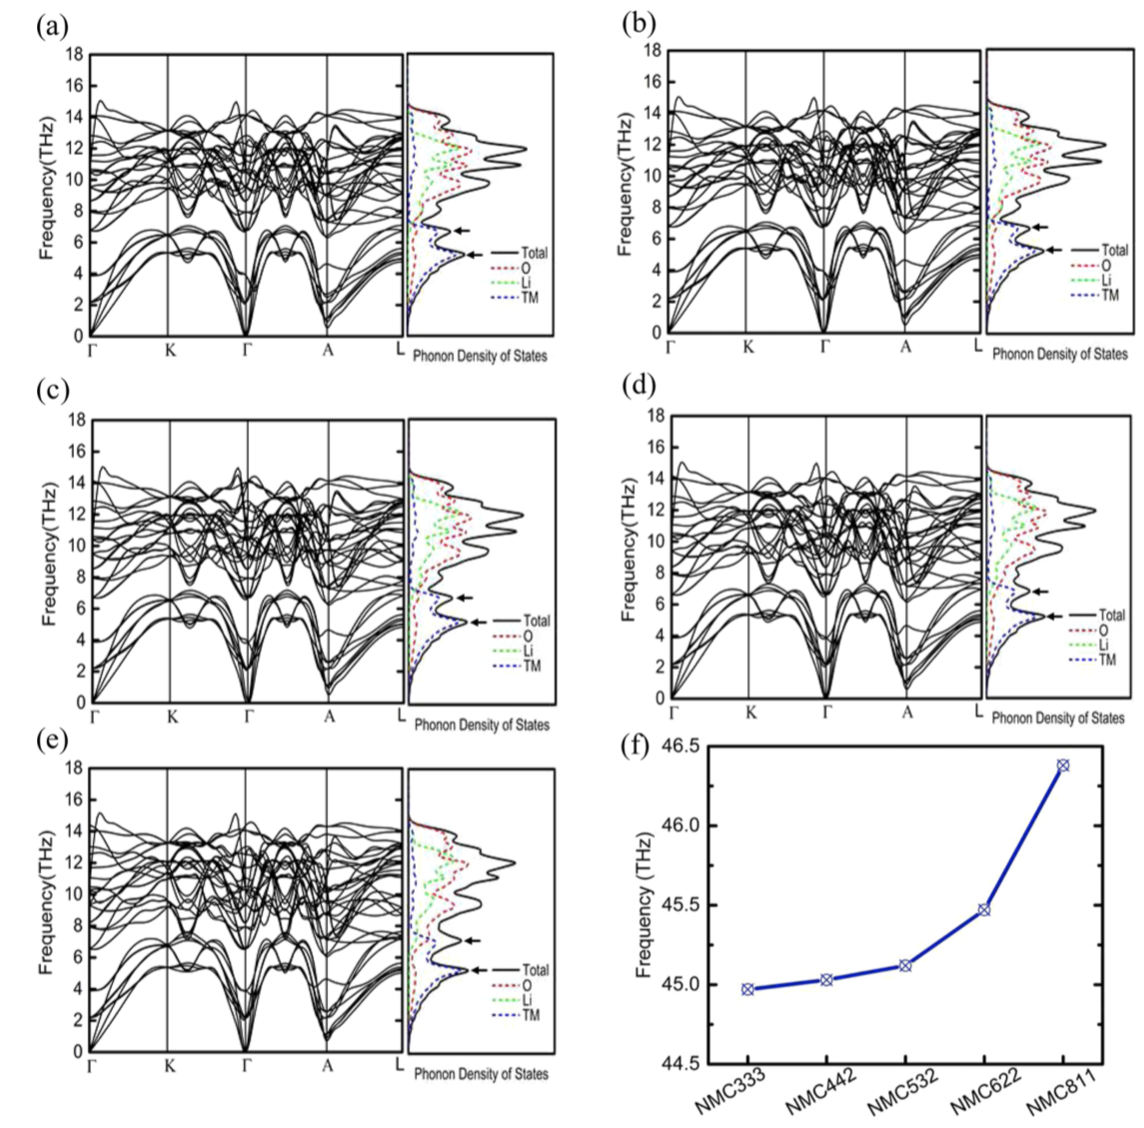
\includegraphics[width=15cm]{Figures/P_phonon.png}
    \caption{(a-e) Phonon dispersion and density of states of NMC333, NMC442, NMC532, NMC622, and NMC811, respectively. DOS curves are showed on the right panel. (f) Longitudional acoustic frequency in the five NMC compounds around the $\Gamma$ point of the Brillouin zone, reproduced with permission from Ref. \citenum{sun_electronic_2017}.}
  \label{figure_phonon}
\end{figure}

%kappa, real device, impact
Both the electrochemical and thermal properties of Li(Ni$_x$Mn$_y$Co$_z$)O$_2$ are dependent on its composition. 
An increase of the Ni content results in an increase in specific discharge capacity and total residual lithium content, however, the corresponding capacity retention and safety characteristics gradually decreased, Figure \ref{figure_thermal}a. \cite{noh2013comparison} 
Increasing Ni/Mn content leads to lattice thermal conductivity suppression.\cite{yang2020chemical}
Thermal conductivity decays exponentially with increasing temperature due to enhanced phonon scattering resulting from the larger thermal population of phonon modes.
Figure \ref{figure_thermal} b shows that at room temperature NMC811 has the lowest predicted thermal conductivity of 9.3 \SI{}{W.m^{-1}.K^{-1}} , while NMC622 and NMC111 are higher at 13.3 and 17.9 \SI{}{W.m^{-1}.K^{-1}}, respectively.
In most devices, the thermal conductivity is much lower than these theoretical upper limit.\cite{takahata2002thermal,chen2006thermal}
Both having smaller grain sizes in poly-crystalline cathode materials and charging (delithiation) softens the lattice leading to smaller phonon velocities and stronger phonon scattering. \cite{feng2020quantum,xia2020high}
These studies show the accessibility of tuning cathode material properties systematically by optimizing the ratio of the transition metals in NMC alloys, overcoming some of the challenges in battery cathode design.

\begin{figure}[]
  \centering
    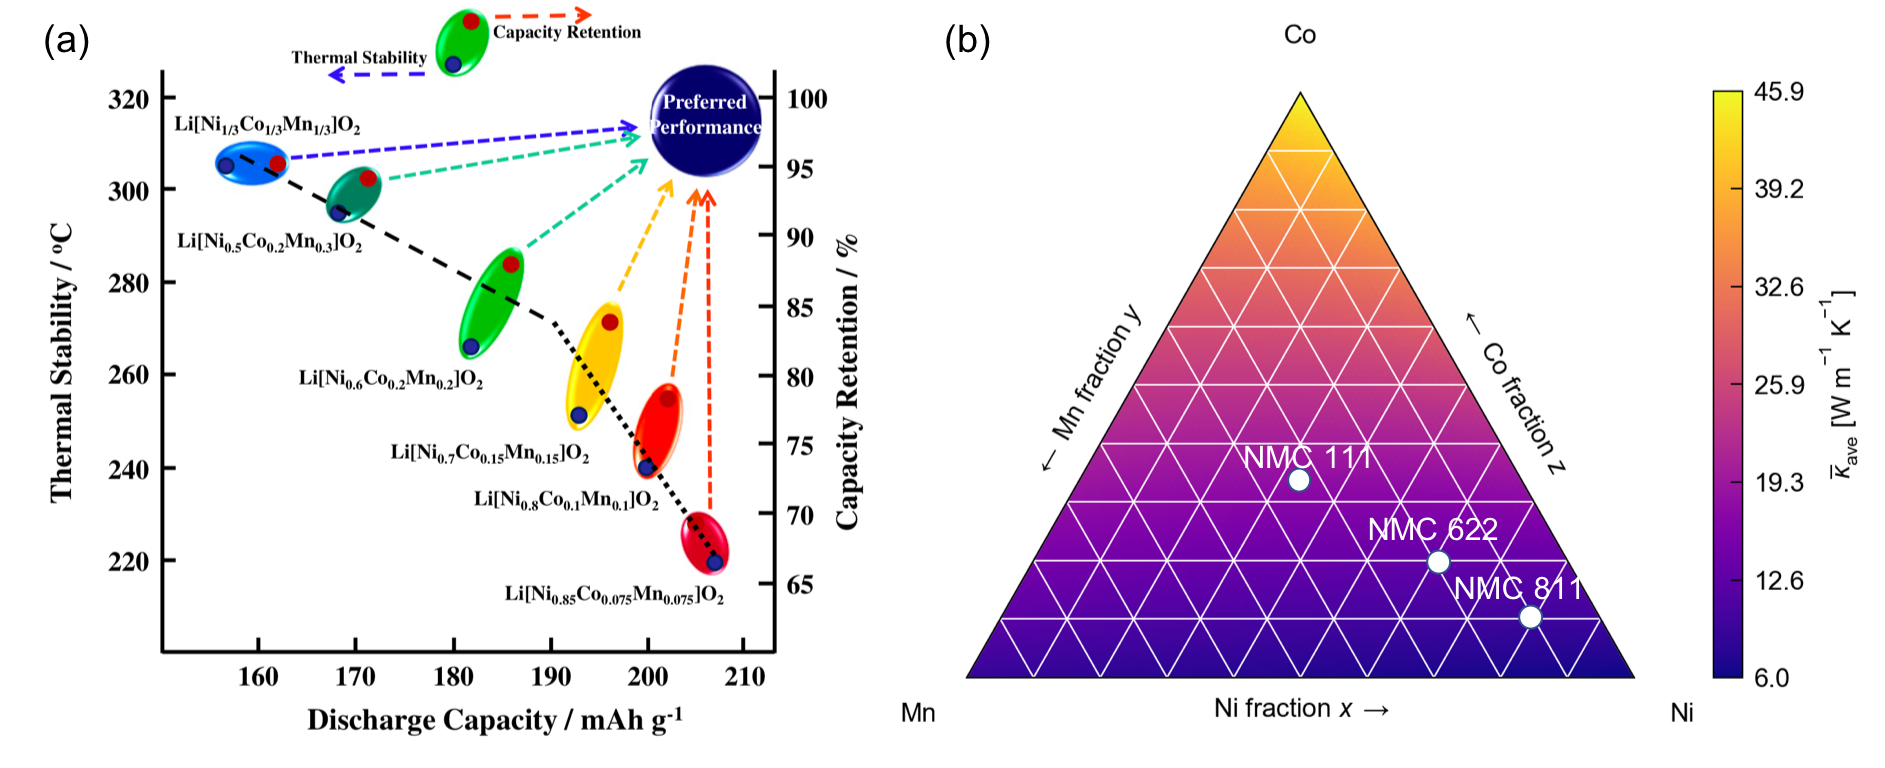
\includegraphics[width=16cm]{Figures/P_thermal.png}
    \caption{(a) Relation between discharge capacity, and thermal stability and capacity retention of Li/Li(Ni$_x$Mn$_y$Co$_z$)O$_2$ (x = 0.33, 0.5, 0.6, 0.7, 0.8 and 0.85), reproduced with permission from Ref. \citenum{noh2013comparison}. (b) Ternary map of the thermal conductivity map $\kappa$ of the NMC system with consideration of mass variation at the cation site, reproduced with permission from Ref. \citenum{yang2020chemical}.}
  \label{figure_thermal}
\end{figure}

%\clearpage
\section*{Cells: Operation and Degradation}
Atomistic modelling is ideal for investigating bulk and localised behaviour, however, these predictions do not provide macroscopic information on material behaviour at the cell level. 
Here, continuum models are well suited to provide further detail. 
These are governed by mathematical expressions that relate concentrations and potentials (partial differential equations). 
Values describing different properties, such as diffusion coefficients and equilibrium potentials are required as inputs or parameters.

The DFN model requires over 25 parameters with the exact number dependent on how the equations are expressed.\cite{Kim2011} 
Parameter estimation can be used to simplify the process. 
The approach requires only voltage and current measurements of the battery to evaluate parameters, removing the need for a cell teardown and extensive characterisation i.e. dismantling the cell to extract the components for analysis. \cite{Jin2018} 
However, this is complicated by the large number of parameters that have to be fitted.
%\subsection{Pararameterisation (Kieran)}
The computational expense currently precludes the use of this model in battery management systems, instead equivalent circuit models are favoured due to their simplicity.\cite{Marquis2019} 
However, the DFN model has been used extensively in battery material development as it provides detailed physical insights compared to other model classes.\cite{Dawson2018}

Recent interest in Ni-rich cathodes has seen the DFN model used extensively to understand the use of graded electrodes (containing multiple electrode particle sizes), to deconvolute capacity and power fade predictions, and to investigate the efficacy of tab and electrode designs for fast charging.\cite{Richardson2020,Kindermann2017,Sturm2019} 
This research has been dependent on parameter sets for NMC materials being reported, however, these values may not reliably describe the properties of Ni-rich NMC because studies may use parameters determined for cathodes with lower/unknown Ni content. 
For example, \citeauthor{Richardson2020} et al. modelled an NMC material using the properties of LiNi$_{0.4}$Co$_{0.6}$O$_2$, directly measured by \citeauthor{Ecker2015}\cite{Richardson2020,Ecker2015} \citeauthor{Kindermann2017} measured the geometry of an NMC\textendash with unknown stoichiometry  \textendash electrode extracted from a Samsung cell.\cite{Kindermann2017} 
Electrode diffusivity and reaction rates were estimated and not evaluated directly, while the equilibrium potential was represented by that of an NMC111 material reported elsewhere.\cite{Stewart_2008} 

Parameterisation is essential for modelling NMC cathode materials, as simulations act as a powerful tool to investigate the properties of NMC and optimise design without the need to conduct resource-intensive experiments.\cite{shearing_2020_3D} 
Previously, several NMC-based (with low nickel content) batteries have been experimentally parameterised. \cite{Ecker2015,Schmalstieg_Rahe_Ecker_Sauer_2018,Liebig_2019} \citeauthor{Ecker2015} reported the physico-chemical properties and anatomy of a LiNi$_{0.4}$Co$_{0.6}$O$_2$ based pouch cell, offering a comparison of different techniques used to evaluate the electrode diffusivity. \cite{Ecker2015} \citeauthor{Schmalstieg_Rahe_Ecker_Sauer_2018} investigated a battery composed of a NMC111 mapping the exchange current density, its activation energy, and electrode diffusivity as a function of lithiation by defining the stoichiometries of each electrode. \cite{Schmalstieg_Rahe_Ecker_Sauer_2018} 
\citeauthor{Liebig_2019} studied the electrochemical behaviour of a large format NMC cell, extending the model predictions to include thermal behaviour. \cite{Liebig_2019} 
These papers outline the cell properties required for simulations and the methods used to determine them. 
These methodologies prove a valuable tool for other groups to undertake similar investigations, by detailing a procedure that can be applied to other materials. 
For modellers investigating high-Ni NMC materials these properties provide limited utility as they do not accurately describe its behaviour. 
This can be attributed to the electrochemical properties being significantly affected by the different crystal structures in NMC materials.\cite{noh2013comparison} 

It is difficult to predict the values of parameters for high-Ni materials based on the determined values for lower Ni-content materials.\cite{Amin_Chiang_2016} 
This is attributed to the presence of different thermodynamic phases compared to NMC811, which affects the dependency of several parameters on the state of lithiation. 
The H2 $\rightarrow$ H3 phase transition above 4.1V has not been reported in NMCs with Ni-contents \textless80\% and can explain parameter differences.\cite{jung2017oxygen} 
Thermodynamic phases in materials are  property-determinant. To address the limited contributions in this context, authors have focused on specifically parameterising NMC811 chemistries. 
\citeauthor{Chen2020} detailed the parameters for a 21700-cylindrical cell, validating and tuning these values for cell discharge.\cite{Chen2020} 
Sturm \& Jossen \textit{et al.} reported a full electrochemical-parameterisation of a DFN model to study lithium plating during fast charging of a NMC-811/SiC cell.\cite{Sturm2019b,Sturm2019} 
It can be time consuming to conduct literature searches to find parameters, to develop the code to simulate battery behaviour, and to collect the data to validate model predictions. 
The availability of software and data has been essential in enabling innovations in this field.

%\subsubsection{Packages}
Traditionally, the sourcing of parameters required an extensive literature search and/or knowledge of prominent authors in the field. 
Recently, the development of databases and software that collate parameter values for battery components have streamlined this process and proved essential in modelling applications. \cite{Tranter2020,Tranter_2020b} 
Wang et al. created a database that details over 100 parameterisations of batteries or the individual components and the techniques that have been used to determine them. 
Additionally, Python Battery Mathematical Modelling (PyBaMM) is a software package that has been explicitly developed for continuum modelling, it caters for multiple definitions and allows the construction of a battery from various component chemistries.\cite{Sulzer_2020} 
These include parameters that describe a commercially-made NMC811 electrode.\cite{Chen2020} 
The parameter set for this material has been utilised in several investigations.\cite{Tranter2020,Tranter_2020b} 
PyBaMM provides a robust approach to modelling of NMC—and other materials—as the electrochemical behaviour can be simulated with only several lines of code (Figure \ref{fig:pybamm}).

Model predictions require validation with experimental data. 
The validation requirements often call for long-term cycling experiments that many institutions do not have the facilities to carry out themselves. 
Providing these data sets via open access repositories means researchers can more readily find the data they require for model development. 
Data availability in science is critical for progress, this is especially true in model development, providing parameter values and raw data improves accessibility and transparency leading to better research throughout the community. 
There are many instances of validation data, we would like to highlight the following. 
\citeauthor{Chen2020} have made available data on the discharge and subsequent relaxation of the NMC811-based cylindrical cell that was used in the validation of the parameter set (Ref.~\citenum{zenodo}). \cite{Chen2020}
\citeauthor{Devie_2018} have provided data sets on the degradation of 18650 cylindrical cells based on NMC, NCA, and LFP chemistries, the study is ongoing and is examining the influence of operating conditions on the ageing of cells (Ref.~\citenum{BatteryArchive}). \cite{Devie_2018}

\begin{figure}[h]
    \centering
    \resizebox{14cm}{!}{\includegraphics*{Figures/pybamm.png}} %
    \caption{\label{fig:pybamm} Screenshot of the Python workflow and results obtained from a PyBaMM battery simulation.} 
\end{figure}

%\subsubsection{Summary}
Parameterisations are a critical exercise in model development, additionally they provide useful insights into the properties of a lithium-ion battery and its components. 
It is important to be aware of the nuances in reported parameter values, specifically that different techniques provide considerably different information and that modelling predictions are most accurate when the parameters have been explicitly determined for the battery being studied. 
The availability of parameters and validation data has proven valuable to the research community, software has been developed in this context. 
For example, PyBaMM has is a powerful tool that connects researchers with parameter sets and robust code.  

The thermal and electrochemical behaviours of battery materials have been widely described, however, being able to accurately predict the degradation has proven more difficult. 
This can be ascribed to the difficulty measuring the required parameters, presently, many of these parameters are assumed or fitted. 

%\subsection{Degradation: Identifying and Predicting (Anisha)}
Experimental characterisation of physical and chemical properties provides essential data for creating accurate parameterisation and validation models that identify and investigate  battery degradation processes. 
Both electrodes are susceptible to a range of degradation modes that effect the impedance, power, and capacity of a cell. 
\citeauthor{Edge2021Degradation} provide a detailed guide to understanding these modes, the mechanisms causing them, and the resulting effects, in order to design experiments or develop models for investigating battery degradation.\cite{Edge2021Degradation} 
There are two key degradation modes for the NMC positive electrode material which directly effect impedance, power, and capacity: loss of lithium inventory (LLI) and loss of active material (LAM), .\cite{erickson2017recent,erickson2017recent}
Repeated cycling causes volume changes that result in particle cracking, \cite{Woodford2010} and leads to loss of contact between particles and the current collector.\cite{erickson2017recent} 
The cathode electrolyte interface (CEI) which has formed in cracks triggers side reactions with the electrolyte, leading to passivation layer formation, consuming lithium ions, i.e. LLI and hence impedance increase.\cite{erickson2017recent}
Operating at high voltages ($\geq$3.7~V) also promotes CEI formation as well as other detrimental surface processes such as gas evolution (O$_{2}$, CO$_{2}$ and CO).\cite{jung2017chemical} 
NMC811 has a higher susceptibility towards oxygen evolution due to its higher nickel content.\cite{Phillip2020} 
Long term cycling, operating at high voltages and temperatures causes dissolution of TMs resulting in LAM and significant capacity fading. \cite{li2018temperature} 
NMC811 has a higher susceptibility, again due to the reactivity of highly oxidised nickel cations with the electrolyte, causing decomposition and resulting in TM dissolution.\cite{billy2018dissolution} 
Accurate prediction of cell behaviour requires monitoring these processes and deciphering the interplay between the processes that take place.
This is done by physical and chemical characterisation, which provides data essential for accurate parameterisation and validation of models, leading towards the design of more realistic models for accurate prediction of cells life.

%\subsubsection{Prediction (Abir)}
Degradation mechanisms of the positive electrode can be investigated using SPM \cite{reniers2019review,jana2019physical} and DFN \cite{lin2013comprehensive} continuum-scale models. 
For example, oxygen evolution from the positive electrode is conventionally modelled as the oxidation of electrolytes at the positive electrode, introducing a simple kinetically limited Tafel equation \cite{lin2013comprehensive,reniers2019review} in the DFN or SPM model. 
\citeauthor{jana2019physical} proposed that the capacity fade is a linear function of the oxidation current density, which the authors used in the Tafel equation to model the electrolyte oxidation at the positive electrode.\cite{jana2019physical} 
However, theoretical understanding and available models for the source of the oxygen evolution and its effect on the capacity fade are not well developed. 
Recently, \citeauthor{ghosh2020shrinking} have proposed a physics-based shrinking core model for the degradation of NMC811 electrodes that undergo a structural reorganisation involving oxygen loss and the formation of a disordered (spinel or rock-salt structure) passivation layer (PL). \cite{ghosh2020shrinking} 
The model considers [O] released from the bulk-PL interface and reaction kinetics of the same control reaction rate. 
Li-entrapment and growth of the PL cause capacity fade. 
Two limiting cases – \textit{`diffusion dominated'} and \textit{`reaction dominated'}, manifest with the variation in the relative rates of [O]-diffusion and [O]-release and the thickness of the PL. 
TM dissolution at the positive electrode is modelled using a first order chemical reaction, limited by the concentration of \ce{H+} ions in the electrolyte. \cite{dai2012capacity} 
\ce{H+} ions are generated from \ce{LiPF6} salt dissociation in the electrolyte and solvent oxidation at the positive electrode. 
While \ce{LiPF6} dissociation in the presence of \ce{H2O} is modelled using a chemical reaction rate, solvent oxidation is modelled using irreversible Butler-Volmer kinetics. \cite{dai2012capacity} 
\citeauthor{lin2013comprehensive} provided detailed DFN model equations for TM dissolution at the PE coupled with SEI layer formation at NE. \cite{lin2013comprehensive} 
The TM deposition on negative electrode is also included in the model. 
The growth of the CEI can be modelled as similar to any of the SEI layer growth models. 

%\subsubsection{Summary}
Key degradation processes that take place at the positive electrode material and their effects have been discussed, as well as fundamental characterisation techniques that aide tracking and monitoring of these processes have been introduced. In order to use models to estimate aging mechanisms during normal or even fast charging, accurate determination of the parameters that describe the physical, chemical, and electrochemical properties of the cell is key. The reliability of models to predict a cells behaviour, which varies between different types of cells, requires experimental data. Electrochemical techniques are fast and practical diagnostic tools used in situ characterisation of battery performance, providing information on capacity, resistance and coulombic efficiency. The use of multiple approaches produces rich data, which is required for cell monitoring, deciphering the degradation processes taking place during cell cycling, and essential for accurate parameterisation and validation of models, leading towards the design of more realistic models for accurate prediction of cells life.

\section*{Summary and Outlook}
% Suggestions from Aron:
% \begin{itemize}
    % \item For electrons - order of oxidation during delithation
    % \item For ions - accurate IPs that can describe redox changes
    % \item For phonons - extending to polycrystalline and nanoparticle structures
    % \item For devices [and cells] - integrating atomic features to produce more general models. Perhaps, a nod to physics-based machine learning as the saviour.
% \end{itemize}

We have reviewed progress in the computer simulation of NMC electrodes from the atomic to the cell scale. Looking at each length scale, a number of outstanding challenges can be identified.
For electronic structure studies, proper elucidation of the oxidation states of mixed TMs in NMC is important for improving its applicability as cathode in LIBs. Layered oxides with high Ni content have three critical challenges: cycle instability, thermal instability, and air instability, all of which are related to the instability of Ni$^{3+}$ or Ni$^{4+}$ in contact with the liquid organic electrolyte or ambient air.\cite{Manthiram-NatComm-2020} The mixed nature of TMs also impacts the thermodynamic stability of NMC materials. Analysis of the thermodynamics to obtain accurate interatomic force constants (IFCs) for the material is crucial. These are extracted acquired through extensive first principles calculations of systematic finite differences. However, this approach scales poorly with system size and structural symmetry and is therefore too expensive to extend beyond third-order IFCs. An alternative method would be to use machine learning (ML) which comprises models that learn from existing large data sets to make predictions. For example, a newly developed package based on ML, hiPhive, enables the efficient extraction from first-principles calculations using regression techniques with regularization.\cite{eriksson2019hiphive}

For molecular dynamics studies, a bottleneck is the availability of an interatomic potential with the ability to accurately describe essential properties for a battery material, such as the redox chemistry. To achieve this, fitting to better training data, and potentially more sophisticated functional forms are needed. Progress has also been made in using machine learning to develop new, more reliable, potentials. \citeauthor{deringer2019machine} recently published a progress update, showing how machine learning is improving interatomic potentials by ``learning'' from electronic-structure data, which give better accuracy in approximating material properties. \cite{deringer2019machine}

Inaccuracies in continuum models have manifested due to the lack of original parameter sets in literature and improper experimental design. Realistic models for predicting cell lifetime and managing operation require a comprehensive understanding of the degradation processes. To obtain representative data, physical and chemical characterisation needs to be carried out. The use of multiple diagnostic tools produces rich data, essential for accurate parameterisation and validation of models, leading towards the design of more realistic models for accurate prediction of cells life. However, information in literature may not be representative of the material being modelled and mistakes can be easily propagated.\cite{Howey_2020} Extensive parameterisation of high Ni content NMC stoichiometries is needed to avoid use of data from lower Ni materials, which are not suitably representative due to dissimilar properties. Further to this, construction of a parameter database would prevent reproduction of errors. Equally important is having a holistic understanding of the experimental techniques and model assumptions. The theory underpinning the experiments used in parameterisation must be consistent with that of the model to make truly robust predictions. There are several research groups around the world currently working towards addressing these problems.

Continuum models of high-nickel electrode degradation are key to reveal the underlying physics of the degradation mechanisms. At the same point of time, whole-cell Li-ion battery models are incomplete without the incorporation of positive electrode degradation mechanisms. In that respect, modelling of individual degradation mechanisms as well as combining them into the whole-cell models is the future goal. Accurate parameterisation is important for the success of these kind of models. Degradation experiments and fundamental molecular-scale and DFT studies are essential for the development of continuum scale whole-cell degradation models.\cite{Sulzer_2020} These models will then be capable of predicting the key conditions to increase the life-time of these batteries.

Connecting continuum and atomistic models predictions can provide a more detailed understanding of the charge and mass transport processes, resulting in more accurate predictions of battery behaviour. Attempts to join the atomistic to the continuum scale have been previously attempted, however, there is no simplistic method for joining the different length scales due to the difference in mathematical principles used in each model.\cite{Fackeldey2015} Continuum models comprise of partial differential equations (PDEs), while atomistic models use discrete models.\cite{Badia2007} This difference in mathematical principles leads to different calculable properties, for example, in atomistic modelling charge transport is related to self-diffusion within the crystal lattice, whereas charge transport in continuum modelling relates to macroscopic diffusion in the electrode, often being experimentally determined. Solutions to overcome this mismatch in calculable properties is of great interest and one of the biggest challenges in obtaining consistent multi-scale models of battery materials.

\bibliography{references}

\end{document}